\chapter{Pendahuluan}
\label{chap:pendahuluan}

\section{Latar Belakang}
\label{sec:latar_belakang}
KIRI\cite{kiritravel} (Gambar \ref{fig:1_kiritravel}) merupakan situs web untuk membantu pengguna menemukan rute transportasi umum ke tempat tujuannya. Dengan memasukkan lokasi awal serta lokasi tujuan pengguna tersebut, situs web KIRI akan memberikan langkah-langkah (contoh: berjalan sejauh berapa meter, menggunakan angkot, dan sebagainya) tercepat untuk sampai ke lokasi tujuan.

\begin{figure}[htbp]
	\centering
		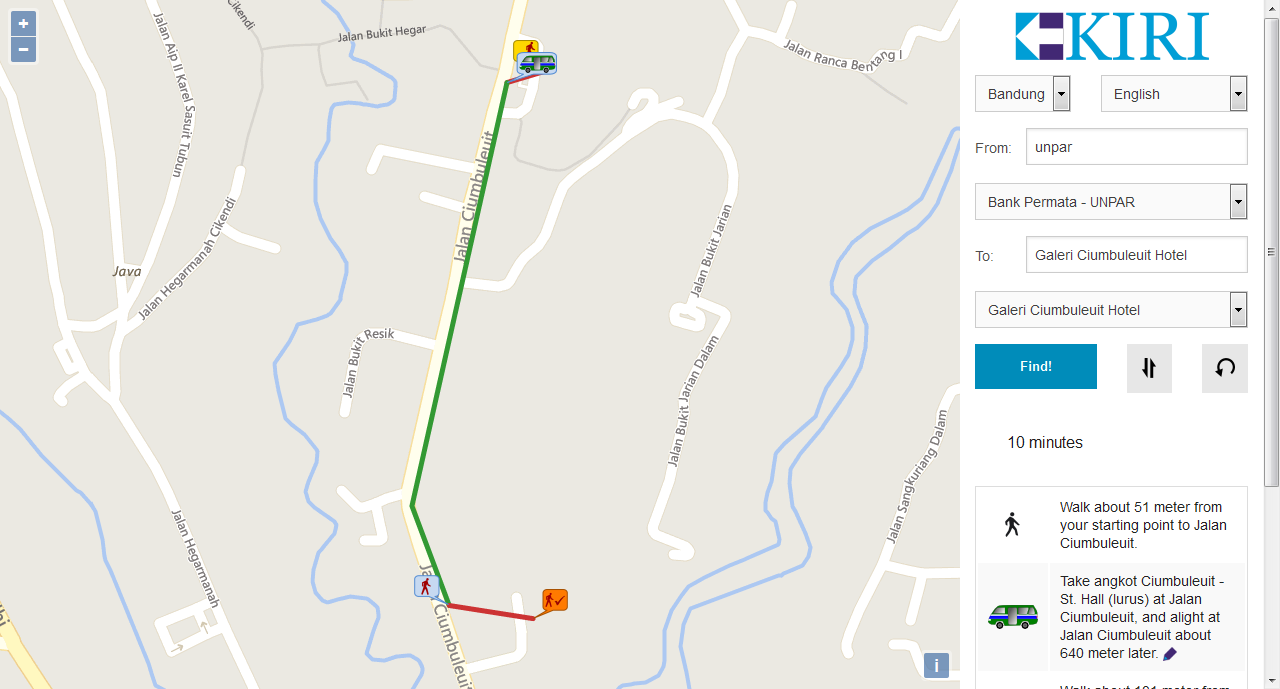
\includegraphics[scale=0.35]{Gambar/1_kiritravel.png}
	\caption{Situs web KIRI\cite{kiritravel}}
	\label{fig:1_kiritravel}
\end{figure}

KIRI \textit{Dashboard}\cite{devkiritravel} (Gambar \ref{fig:1_kiridashboard}) adalah bagian dari situs web KIRI. KIRI \textit{Dashboard} hanya dapat diakses oleh tim developer KIRI. KIRI \textit{Dashboard} berfungsi sebagai pengatur proses CRUD (\textit{Create, Read, Update,} dan \textit{Delete}) data pribadi pengguna (tim developer), daftar rute angkutan umum, dan API \textit{keys} yang terdapat dalam \textit{database} situs web KIRI. KIRI \textit{Dashboard server side} menggunakan bahasa PHP dalam pembuatannya\cite{kiridashboard}. Bahasa PHP kurang cocok untuk proyek skala besar seperti \textit{dashboard}. Salah satu penyebab bahasa PHP kurang cocok adalah karena tidak ada deklarasi dan tipe variabel dalam penggunaan bahasa PHP.

Tidak ada deklarasi dan tipe variabel dalam PHP dapat menyebabkan suatu kesalahan yang tidak terduga. Kesalahan tipe data variabel dapat terjadi pada saat memberikan nilai ataupun pemanggilan fungsi (kesalahan tipe variabel pada parameter). Contoh permasalahannya adalah terdapat 2 buah konstanta, konstanta pertama bertipe \textit{Integer} dan konstanta kedua bertipe \textit{String} (seharusnya bertipe \textit{Integer} juga), maka jika melakukan eksekusi penjumlahan antara konstanta pertama dan kedua tetap dapat dilakukan dalam PHP, namun hasilnya tidak sesuai dengan yang diharapkan.

Java merupakan bahasa pemrograman yang umum digunakan oleh banyak orang. Selain umum digunakan, Java juga merupakan bahasa pemrograman yang lebih terstruktur dibandingkan dengan PHP. Adanya deklarasi dan tipe variabel pada Java membuat setiap variabel memiliki kegunaan yang jelas dan dapat mencegah terjadinya kesalahan seperti yang telah dijelaskan. Play Framework merupakan salah satu \textit{framework} yang membantu implementasi Java dalam pembuatan suatu situs web. Play Framework menggunakan konsep arsitektur MVC (\textit{Model View Controller})\cite{playforjava} pada struktur kodenya. Arsitektur MVC memisahkan bagian struktur data (\textit{model}) dan tampilan (\textit{view}) sehingga proses pengembangan dapat dilakukan lebih cepat (tidak saling ketergantungan).

\begin{figure}[htbp]
	\centering
		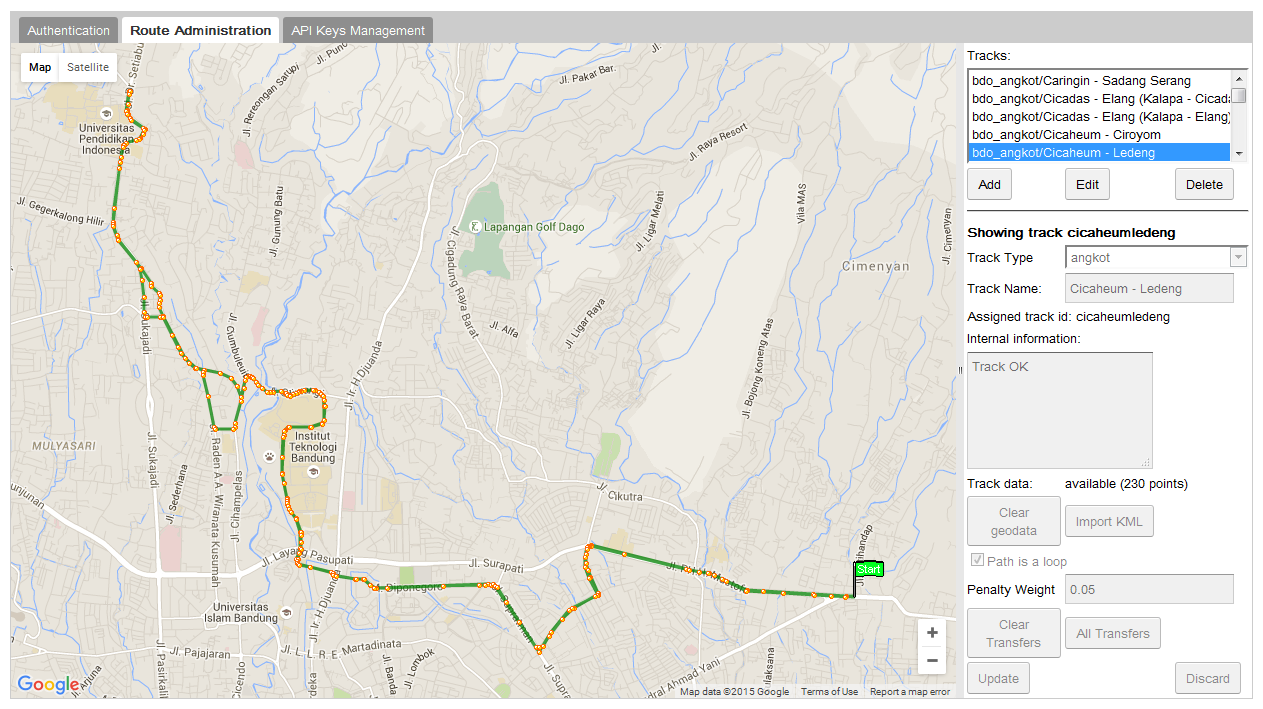
\includegraphics[scale=0.35]{Gambar/1_kiridashboard.png}
	\caption{KIRI \textit{Dashboard}\cite{devkiritravel}}
	\label{fig:1_kiridashboard}
\end{figure}

Berdasarkan ditemukannya kekurangan-kekurangan pada KIRI \textit{Dashboard server side} seperti yang telah dijelaskan, maka solusi untuk mengatasi kekurangan tersebut adalah dibuatlah penelitian ini untuk mengubah KIRI \textit{Dashboard server side} yang semula dalam bahasa PHP menjadi bahasa Java dengan menggunakan Play Framework tanpa mengurangi keseluruhan fungsi yang dimiliki.

\section{Rumusan Masalah}
\label{sec:rumusan_masalah}
Berikut adalah susunan permasalahan yang akan dibahas pada penelitian ini:
	\begin{enumerate}
		\item Bagaimana isi kode KIRI \textit{Dashboard server side}?
		\item Bagaimana melakukan \textit{porting} KIRI \textit{Dashboard server side} yang semula dalam bahasa PHP menjadi bahasa Java dengan menggunakan Play Framework?
		\item Bagaimana perbandingan waktu eksekusi antara KIRI \textit{Dashboard server side} yang dibangun dengan PHP dan KIRI \textit{Dashboard server side} yang dibangun dengan Play Framework?
	\end{enumerate}
	
\section{Tujuan}
\label{sec:tujuan}
Berdasarkan rumusan masalah yang telah dibuat, maka tujuan penelitian ini dijelaskan ke dalam poin-poin sebagai berikut:
	\begin{enumerate}
		\item Mengetahui isi kode KIRI \textit{Dashboard server side}.
		\item Melakukan \textit{porting} KIRI \textit{Dashboard server side} yang semula dalam bahasa PHP menjadi bahasa Java dengan menggunakan Play Framework.
		\item Mengetahui perbandingan waktu eksekusi antara KIRI \textit{Dashboard server side} yang dibangun dengan PHP dan KIRI \textit{Dashboard server side} yang dibangun dengan Play Framework.
	\end{enumerate}
	
\section{Batasan Masalah}
\label{sec:batasan_masalah}
Penelitian ini dibuat berdasarkan batasan-batasan sebagai berikut:
	\begin{enumerate}
		\item Play Framework yang digunakan selama penelitian ini adalah versi 2.4.3.
		\item \textit{Porting} Kode KIRI \textit{Dashboard server side} yang dilakukan adalah berdasarkan URL \url{https://github.com/pascalalfadian/tirtayasagh}, \textit{commit number:} b650bfa.
	\end{enumerate}
	
\section{Metode Penelitian}
\label{sec:metode_penelitian}
Berikut adalah metode penelitian yang digunakan dalam penelitian ini:
	\begin{enumerate}
		\item Melakukan studi literatur mengenai kode KIRI \textit{Dashboard server side}, MySQL Spatial Extensions, JDBC, Play Framework, JSON, dan \textit{Regular Expression}.
		\item Menganalisis teori-teori untuk membangun KIRI \textit{Dashboard server side} dalam bahasa Java dengan menggunakan Play Framework.
		\item Merancang KIRI \textit{Dashboard server side} dalam bahasa Java dengan menggunakan Play Framework.
		\item Melakukan \textit{porting} kode situs web KIRI \textit{Dashboard server side} menjadi Java dengan menggunakan Play Framework.
		\item Melakukan pengujian terhadap fitur-fitur yang sudah dibuat.
	\end{enumerate}

\section{Sistematika Penulisan}
\label{sec:sistematika_penulisan}
Setiap bab dalam penelitian ini memiliki sistematika penulisan yang dijelaskan ke dalam poin-poin sebagai berikut:
	\begin{enumerate}
		\item Bab 1: Pendahuluan, yaitu membahas mengenai gambaran umum penelitian ini. Berisi tentang latar belakang, rumusan masalah, tujuan, batasan masalah, metode penelitian, dan sistematika penulisan.
		\item Bab 2: Dasar Teori, yaitu membahas mengenai teori-teori yang mendukung berjalannya penelitian ini. Berisi tentang MySQL Spatial Extensions, JDBC, Play Framework, JSON, dan \textit{Regular Expression}.
		\item Bab 3: Analisis, yaitu membahas mengenai analisa masalah. Berisi tentang analisis sistem kini, analisis tampilan sistem kini, analisis \textit{database} sistem kini, analisis sistem usulan, dan analisis \textit{libraries} sistem usulan.
		\item Bab 4: Perancangan, yaitu membahas mengenai perancangan yang dilakukan sebelum melakukan tahapan implementasi. Berisi tentang perancangan kelas dan pemodelan KIRI \textit{Dashboard} dalam Play Framework.
		\item Bab 5: Implementasi dan Pengujian, yaitu membahas mengenai implementasi dan pengujian aplikasi yang telah dilakukan. Berisi tentang implementasi dan hasil pengujian aplikasi.
		\item Bab 6: Kesimpulan dan Saran, yaitu membahas hasil kesimpulan dari keseluruhan penelitian ini dan saran-saran yang dapat diberikan untuk penelitian berikutnya.
	\end{enumerate}